% ============================================================================
% Appendix A: the smooth model of the m_hh spectrum and its uncertainty.
% To be \input after \appendix in the paper (JHEP). Figures: fig_basis.pdf,
% fig_A_*.pdf, fig_spectra_dz.pdf (scripts in docs/paper). References:
% appendices_refs.bib. Comments "% TODO main text" mark references to sections
% of the main text, whose labels are not yet known.
% ============================================================================
\section{The model of the $m_{hh}$ spectrum}
\label{app:A}

This appendix describes the model of the gluon-fusion di-Higgs spectrum used in this paper: how it
is built and fitted to the POWHEG spectra, how its uncertainty is obtained, including a systematic
uncertainty, and how both are validated on spectra not used in the fit. A second, independent model
of the same quantity is described in appendix~\ref{app:B}.

\subsection{The form of the cross section and the data}
\label{app:A:data}

For the HEFT parameters $\theta = (\kappa_\lambda, c_t, c_{tt}, c_{ggh}, c_{gghh})$ the differential cross
section at NLO in QCD has the form~\cite{Buchalla:2018yce,Alasfar:2023xpc}
\begin{equation}
  \frac{d\sigma}{dm_{hh}}(m_{hh};\theta) = \sum_{i=1}^{23} C_i(\theta)\, a_i(m_{hh}),
  \label{eq:A:form}
\end{equation}
where the $C_i$ are known monomials in $\theta$ (products of the coupling factors of the amplitude) and
the coefficient functions $a_i$ depend on $m_{hh}$ only. Equation~(\ref{eq:A:form}) is exact provided that
nothing else in the calculation depends on $\theta$ (scales, parton distributions and cuts are the same
for every $\theta$). The task is to determine the 23 functions $a_i(m_{hh})$.

The data are POWHEG spectra at $\sqrt{s} = 13$~TeV, each at a different point $\theta$ % TODO main text: section describing the samples
in bins of 15~GeV, of which we use the 80 bins between $m_{hh} = 255$ and 1455~GeV. Each spectrum
is a histogram of 40,000 generated events of equal weight $q_s$ (a few incomplete runs have fewer),
so that the cross section in bin $k$ is exactly $t_{sk} = q_s n_{sk}$ with an integer count $n_{sk}$. We
recover $q_s$ and the counts of every spectrum as the greatest common divisor of its bin contents. The
counts are Poisson distributed and, up to a negligible multinomial correlation, independent; near
threshold a bin holds about 1,000--1,800 events, at 1.4~TeV about 20. One thousand spectra are set aside
as \emph{test spectra} and play no part in any fit. The bins of the remaining 3,989 spectra are split at
random: 88\% (281,044 bins, including 1,814 empty ones) are used in the fit, and the other 12\% (38,076
bins, the \emph{held-out bins}) are used only to determine the systematic uncertainty of
section~\ref{app:A:syst}.

\subsection{The model}
\label{app:A:model}

Each coefficient function is expanded in $J = 40$ cubic B-splines~\cite{deBoor:1978} $B_j$ and multiplied
by the two-body threshold factor $\phi$,
\begin{equation}
  a_i(m) = \phi(m)\sum_{j=1}^{J}\beta_{ij}B_j(m), \qquad \phi(m) = \sqrt{1 - \frac{4m_h^2}{m^2}},
  \label{eq:A:spline}
\end{equation}
with $m_h = 125$~GeV. The factor $\phi$, the velocity of the Higgs bosons in their rest frame, makes the
density vanish at threshold as two-body phase space does, so that the splines describe only the smooth
remainder. The 38 interior breakpoints are uniform in $\sqrt{m - 2m_h}$ between 250 and 1500~GeV, and so
are densest just above threshold, where the spectra change fastest (figure~\ref{fig:A:basis}). The
prediction for a bin is the \emph{integral} of eq.~(\ref{eq:A:form}) over the bin, not its value at the
bin centre:
\begin{equation}
  f_{sk} = \int_{\text{bin }k}\frac{d\sigma}{dm}(m;\theta_s)\,dm
  = \sum_{i=1}^{23}\sum_{j=1}^{J} C_i(\theta_s)\,\beta_{ij}\,I_{jk}, \qquad
  I_{jk} = \int_{\text{bin }k}\phi(m)B_j(m)\,dm .
  \label{eq:A:linear}
\end{equation}
The model is therefore a genuine density in $m_{hh}$, and it is \emph{linear} in its $23J = 920$
parameters $\beta_{ij}$. The integrals $I_{jk}$ are computed once by Gauss--Legendre quadrature. With
one box-shaped basis function per bin in place of the splines, eq.~(\ref{eq:A:linear}) becomes a fit of 23
independent numbers per bin. This \emph{free fit} describes the data as well as any model of the
form~(\ref{eq:A:form}) can, and serves as the benchmark below.

\begin{figure}[!htbp]
\centering
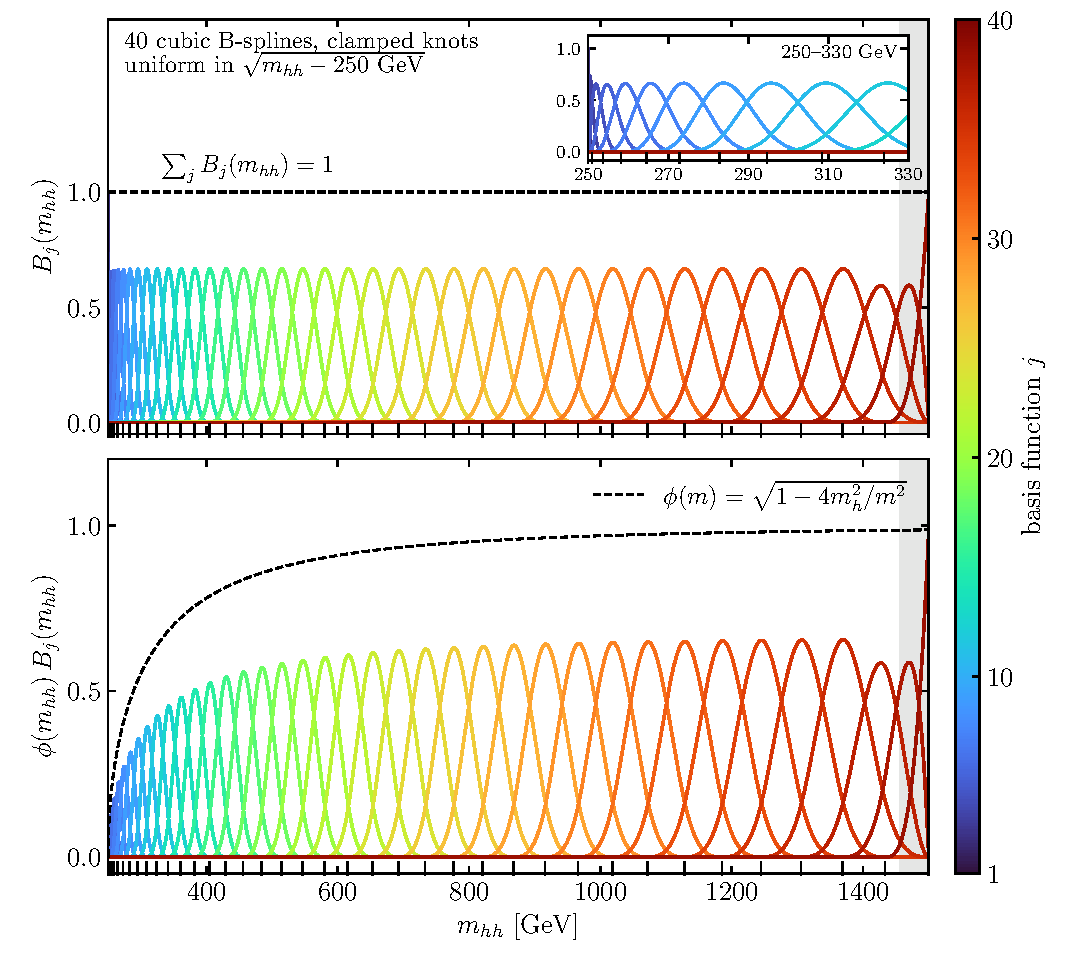
\includegraphics[width=\textwidth]{fig_basis.pdf}
\caption{The basis of the model. Top: the 40 cubic B-splines $B_j(m_{hh})$, coloured by index $j$, with
their breakpoints (ticks), uniform in $\sqrt{m_{hh} - 250~\text{GeV}}$; the inset shows 250--330~GeV.
The splines sum to one everywhere. Bottom: the products $\phi(m_{hh})B_j(m_{hh})$ that multiply the
coefficients $\beta_{ij}$, with the threshold factor $\phi$ (dashed). The shaded region lies beyond the
last bin used.}
\label{fig:A:basis}
\end{figure}

\subsection{Fit and posterior}
\label{app:A:fit}

\paragraph{Likelihood.} With hundreds of events in most bins a Gaussian likelihood with the Poisson
variance is accurate, but the variance must be that of the model's prediction, $q_s\max(f_{sk}, q_s)$, not
that of the observed count. Weighting each bin by $1/(q_s n_{sk})$ (Neyman's $\chi^2$) gives downward
fluctuations larger weights and biases the fit low by about one event per bin~\cite{Baker:1983tu}, which,
with thousands of spectra pooled, is many standard deviations at high mass. We therefore iterate: fit,
recompute the variances from the fit, and refit~\cite{Green:1984}. At convergence this is the Poisson
maximum-likelihood fit.

\paragraph{Smoothness prior.} For each function we use a Gaussian prior on the second differences of its
coefficients~\cite{Eilers:1996},
\begin{equation}
  -\ln\pi(\boldsymbol\beta_i\mid\lambda_i) = \tfrac12\lambda_i\sum_{j=3}^{J}\big(\beta_{ij} - 2\beta_{i,j-1} +
  \beta_{i,j-2}\big)^2 + \text{const},
\end{equation}
plus a negligible ridge term, the discrete analogue of a penalty on the curvature $\int (a_i'')^2\,dm$. The
23 strengths $\lambda_i$ are chosen by maximising the evidence~\cite{MacKay:1992}, which is available in
closed form because the model is linear.

\paragraph{Posterior.} Likelihood and prior being Gaussian in $\boldsymbol\beta$, the posterior is
\emph{exactly} Gaussian, with mean $\hat{\boldsymbol\beta} = H^{-1}\Phi^{\mathsf T}W\boldsymbol t$ and
covariance $H^{-1}$, where $H = \Phi^{\mathsf T}W\Phi + \Lambda$, $\Phi$ is the design matrix of
eq.~(\ref{eq:A:linear}), $W$ the diagonal matrix of inverse variances and $\Lambda$ the prior precision.
Because the monomials and the bins factorise, $\Phi^{\mathsf T}W\Phi = \sum_k S_k\otimes\boldsymbol
I_k\boldsymbol I_k^{\mathsf T}$ with $S_k = \sum_s w_{sk}\boldsymbol C_s\boldsymbol C_s^{\mathsf T}$, and the
whole fit takes about a minute on a laptop. The data determine about 600 of the 920 parameter
combinations; the prior fixes the rest. Predictions for any binning, the density at any $m_{hh}$, the
coefficient functions and the correlations between bins all follow from $\hat{\boldsymbol\beta}$ and
$H^{-1}$. The \emph{fit uncertainty} of a bin is small, a median 2.9\% of the Poisson noise of a POWHEG
bin. Nothing changes, within 0.01 in any measure below, for $J = 30$ or 60.

\subsection{Systematic uncertainty: the model-error term}
\label{app:A:syst}

The comparison of a prediction $f_{sk}$ with a POWHEG bin $t_{sk}$ involves three uncertainties: the
Poisson noise of the POWHEG sample, $s^2_\text{noise} = q_s\max(f_{sk},q_s)$; the fit uncertainty of the
model, $s^2_\text{fit}$; and a third, systematic uncertainty, which arises not from statistical
fluctuations but from the fact that the POWHEG spectra do not exactly obey eq.~(\ref{eq:A:form}). We
describe the evidence for it, its form, and how it is determined. It measures the internal consistency of
the simulated spectra; the uncertainties of the NLO prediction itself (scales, parton distributions, the
top-mass scheme) are separate and are not included. % TODO main text: where theory uncertainties are treated

\paragraph{The evidence.} The accuracy of a prediction $\mu = f/q$ for a count $n = t/q$ is measured by the
likelihood-ratio statistic
\begin{equation}
  -2\ln\lambda = -2\ln\frac{\mathrm{Poisson}(n;\mu)}{\mathrm{Poisson}(n;n)} = 2\left[\mu - n + n\ln\frac{n}{\mu}\right],
  \label{eq:A:lr}
\end{equation}
which for a correct prediction follows, asymptotically, a $\chi^2$ distribution with one degree of
freedom~\cite{Wilks:1938}, with mean 1; no parameter is adjusted to the test spectra. Below 555~GeV its mean
over the test spectra is 1.57, for the smooth model and for the free fit alike (table~\ref{tab:A:accuracy}).
Since the free fit is the best any model of the form~(\ref{eq:A:form}) can do, the excess over 1 is a property
of the spectra, not of the model. It depends on how strongly the 23 terms cancel. With the
\emph{cancellation ratio} of a spectrum, $R_s = \sum_k t_{sk}/\sum_k\sum_i|C_i(\theta_s)A_{ik}|$, where $A_{ik}$ is
the integral of $a_i$ over bin $k$, the fifth of the test spectra with the strongest cancellation
($R < 0.12$) has $\langle z^2\rangle = 1.70$ for the pulls with noise and fit uncertainty only, against 1.01 for
the fifth with the weakest ($R > 0.73$). In the strongest-cancelling fifth the residuals of neighbouring bins
are correlated (0.60 below 555~GeV), so the departures are smooth in $m_{hh}$; Poisson noise would give no
correlation.

\paragraph{The form.} Suppose that in the spectrum of run $s$ each of the 23 terms carries a small relative
error $\delta_i(m;s)$. The error of the spectrum, $\sum_iC_ia_i\delta_i$, is then of order
$\varepsilon\sum_i|C_ia_i|$ for errors of typical size $\varepsilon$, while the cross section is $\sum_iC_ia_i$:
the relative error is amplified by $1/R$ where the terms cancel. The errors must also differ from run to run,
since errors common to all runs would be absorbed into the $a_i$. We therefore add to the variance of each
predicted bin the \emph{model-error term}
\begin{equation}
  s^2_\text{model} = \Big(\varepsilon(m_k)\sum_{i=1}^{23}\big|C_i(\theta)\,A_{ik}\big|\Big)^2 ,
  \label{eq:A:syst}
\end{equation}
in the spirit of the model discrepancy of Kennedy and O'Hagan~\cite{Kennedy:2001}. By the triangle inequality,
eq.~(\ref{eq:A:syst}) is the largest spread that relative errors of size $\varepsilon$ can produce, whatever their
correlation; for independent errors the sum would be taken in quadrature. Both forms calibrate the test spectra
equally well (table~\ref{tab:A:calibration}); we adopt the more conservative one. A systematic proportional to
the Poisson noise instead calibrates the average but not the cancelling spectra.

\paragraph{Determination.} In each bin, $\varepsilon_k$ is fixed on the held-out bins by requiring the pulls
$z = (t - f)/\sqrt{s^2_\text{noise} + s^2_\text{fit} + s^2_\text{model}}$ to have unit variance; $\ln\varepsilon$
is then smoothed by a quadratic in $m_{hh}$, so that the term has three parameters in all
(figure~\ref{fig:A:syst}). It rises from 0.08\% at threshold to 0.28\% at 600~GeV and 3.7\% at 1.45~TeV: near
threshold the 23 components of the POWHEG spectra are consistent to about one part in a thousand. The
model-error term is treated as independent between bins; the residual correlations above show that this is an
approximation, which matters for sums over many bins (section~\ref{app:A:use}).

\begin{figure}[!htbp]
\centering
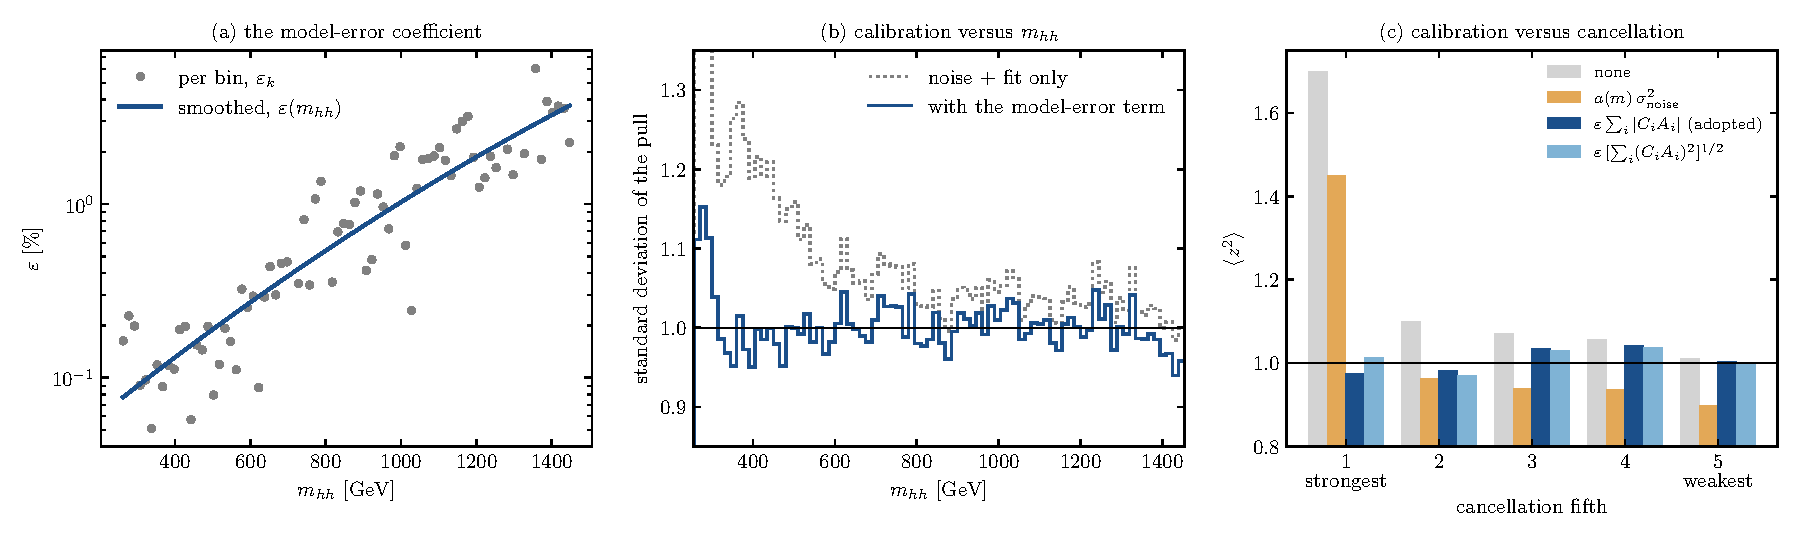
\includegraphics[width=\textwidth]{fig_A_model_error.pdf}
\caption{The model-error term. (a) The coefficient $\varepsilon$: per bin, from the held-out bins (points), and
its three-parameter smooth form (line). (b) Standard deviation of the pull on the 1,000 test spectra in each bin,
without (dotted) and with (solid) the model-error term. (c) $\langle z^2\rangle$ by fifth of the cancellation
ratio, for no systematic, a systematic proportional to the Poisson noise, and the model-error term summed
linearly (eq.~(\ref{eq:A:syst}), adopted) and in quadrature. Each was determined on the held-out bins.}
\label{fig:A:syst}
\end{figure}

\subsection{Validation on the test spectra}
\label{app:A:validation}

\begin{table}[!htbp]
\centering
\small
\begin{tabular}{lccc}
\toprule
 & \multicolumn{2}{c}{mean $-2\ln\lambda$ per bin} & median \\
 & 255--555 GeV & $>555$ GeV & per spectrum \\
\midrule
smooth model                 & 1.566 & 1.100 & 1.078 \\
free fit (benchmark)         & 1.559 & 1.105 & 1.075 \\
\bottomrule
\end{tabular}
\caption{Accuracy on the 1,000 test spectra: the mean of the likelihood-ratio statistic (\ref{eq:A:lr}) per bin,
which is 1 for a perfect model, and the median over spectra of its mean per bin.}
\label{tab:A:accuracy}
\end{table}

\begin{table}[!htbp]
\centering
\small
\setlength{\tabcolsep}{3.5pt}
\begin{tabular}{lccccc}
\toprule
 & \multicolumn{3}{c}{s.d.\ of the pull} & & $\langle z^2\rangle$ by fifth of cancellation\\
systematic & all & 255--555 & $>555$ GeV & $|z|<2$ & (strongest \dots\ weakest)\\
\midrule
none                                     & 1.090 & 1.218 & 1.043 & 93.9\% & 1.70, 1.10, 1.07, 1.06, 1.01\\
proportional to the noise                & 1.018 & 1.049 & 1.008 & 95.3\% & 1.45, 0.96, 0.94, 0.94, 0.90\\
model-error term, eq.~(\ref{eq:A:syst})  & 1.004 & 1.011 & 1.001 & 95.4\% & 0.97, 0.98, 1.04, 1.04, 1.00\\
the same, summed in quadrature           & 1.005 & 1.011 & 1.003 & 95.4\% & 1.01, 0.97, 1.03, 1.04, 1.00\\
\bottomrule
\end{tabular}
\caption{Calibration on the test spectra. For a standard normal, $|z|<2$ holds for 95.4\%. Each systematic was
determined on the held-out bins.}
\label{tab:A:calibration}
\end{table}

\paragraph{Accuracy.} The smooth model reaches the floor set by the free fit: the mean $-2\ln\lambda$ per bin is
1.566 below and 1.100 above 555~GeV (table~\ref{tab:A:accuracy}, figure~\ref{fig:A:accuracy}). The excess over 1 is
the departure described in section~\ref{app:A:syst}, largest just above threshold and for the most cancelling
spectra. Figure~\ref{fig:A:spectra} shows three test spectra, one for each degree of cancellation.

\begin{figure}[!htbp]
\centering
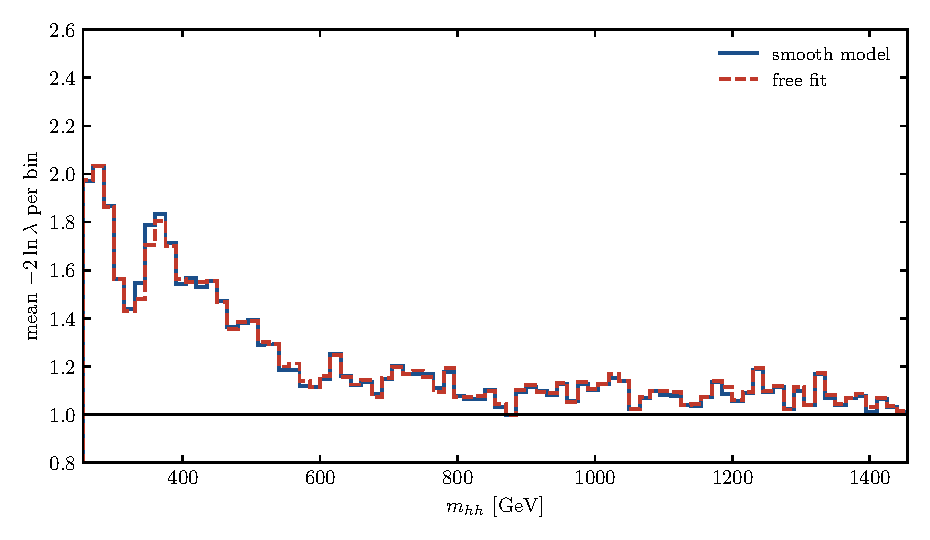
\includegraphics[width=0.72\textwidth]{fig_A_accuracy.pdf}
\caption{Mean likelihood-ratio statistic $-2\ln\lambda$ per bin on the test spectra as a function of $m_{hh}$, for
the smooth model and the free fit; 1 for a perfect model.}
\label{fig:A:accuracy}
\end{figure}

\paragraph{Calibration.} With the model-error term the pulls have unit standard deviation within 1\%, overall,
below and above 555~GeV, and at every degree of cancellation (table~\ref{tab:A:calibration},
figure~\ref{fig:A:syst}). The total predictive uncertainty is a median 1.014 times the Poisson noise of a POWHEG
bin (1.08 in the most cancelling fifth). The pulls of the two lowest bins, 255--285~GeV, where the spectra rise most
steeply, have slightly larger standard deviations (1.11 and 1.15).

\begin{figure}[!htbp]
\centering
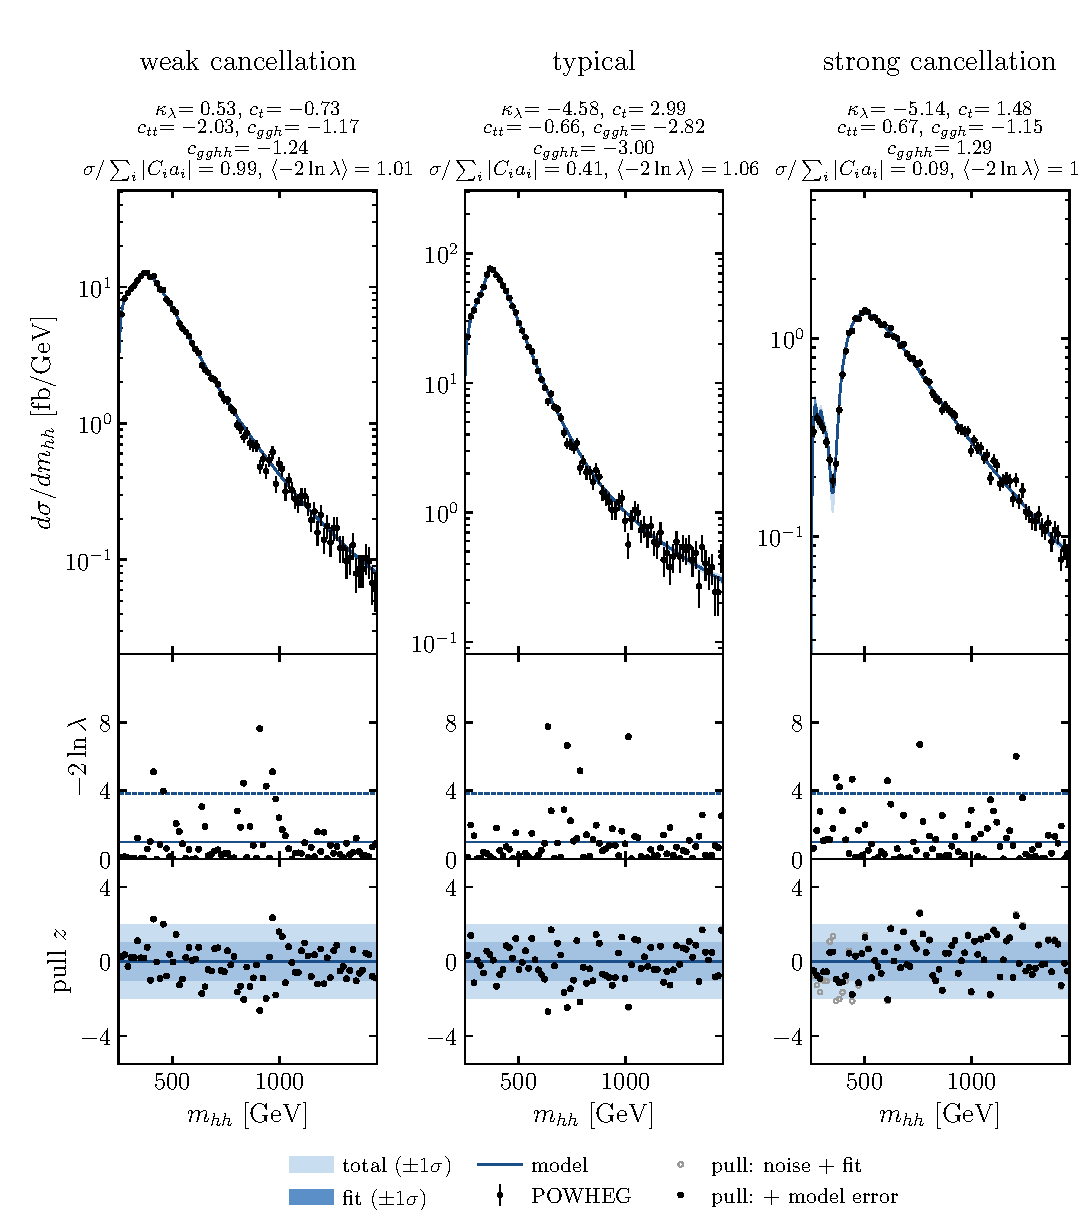
\includegraphics[width=\textwidth]{fig_spectra_dz.pdf}
\caption{Three of the 1,000 test spectra, chosen by how strongly their 23 terms cancel: weak
($R \approx 1$), typical and strong; in each case the spectrum with the median $-2\ln\lambda$ within its fifth of
the cancellation distribution. Top: POWHEG (points) and the model with its fit and total ($\pm1\sigma$) bands.
Middle: $-2\ln\lambda$ per bin, with its mean (1, solid) and 95\% point (3.84, dashed) for a correct model. Bottom:
the pull with the total uncertainty (filled) and without the model-error term (open).}
\label{fig:A:spectra}
\end{figure}

\paragraph{Inside a bin.} To test the model as a density, we fitted it to the training spectra merged into 30~GeV
bins (pairs of 15~GeV bins, whose counts add) and predicted the 15~GeV bins of the test spectra. The measure is the
$\chi^2$ of the difference between the two halves of each pair, in units of its Poisson noise. Above about 360~GeV the
model predicts the split within the noise ($\chi^2$ per pair 1.17 on average between 360 and 555~GeV, at most 1.31;
figure~\ref{fig:A:merged}), as well as the model fitted to the 15~GeV bins does; the free fit, which can only give
each half the same value, gives 7.9 on average there and up to 34 just above threshold. In the first three pairs,
255--345~GeV, the $\chi^2$ is 11, 3.9 and 4.1: the threshold rise has structure on scales finer than 30~GeV, which
30~GeV bins do not fully determine.

\begin{figure}[!htbp]
\centering
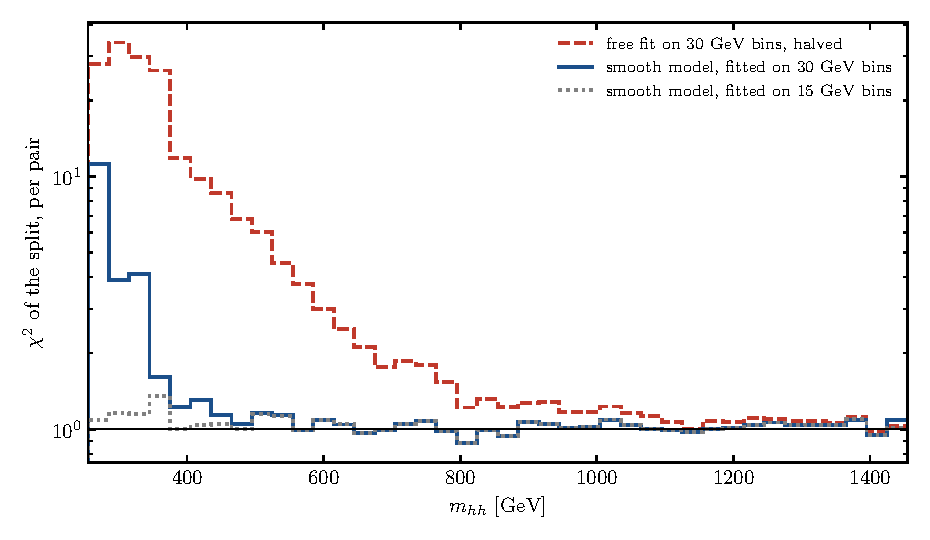
\includegraphics[width=0.72\textwidth]{fig_A_merged.pdf}
\caption{Inside a bin: the model fitted to 30~GeV bins predicts the 15~GeV bins of the test spectra. Shown is the
$\chi^2$ per pair of the split of each 30~GeV bin into its two halves, in units of its Poisson noise (1 is
perfect), for the smooth model fitted to 30~GeV bins, the free fit (each half given half), and the smooth model
fitted to the 15~GeV bins.}
\label{fig:A:merged}
\end{figure}

\paragraph{The edges.} The POWHEG spectra also contain the bins 240--255 and 1455--1500~GeV, not used in the fit.
Summed over the test spectra, the model predicts the first 7\% high (with the factor $\phi$; 55\% high without it).
Above 1455~GeV the splines are fixed by the prior alone and the extrapolation is unreliable. The model should be used
on 250--1455~GeV only.

\subsection{The coefficient functions}
\label{app:A:coefficients}

Figure~\ref{fig:A:coefficients} shows the 23 functions with their exact $\pm1\sigma$ bands. They are smooth and defined
at every $m_{hh}$. The functions whose monomials are small or nearly degenerate over the sampled $\theta$,
$a_{16}$--$a_{20}$, are the least well determined (median relative uncertainty 21--74\%); their uncertainties are
exact and propagate correctly into every prediction.

\begin{figure}[p]
\centering
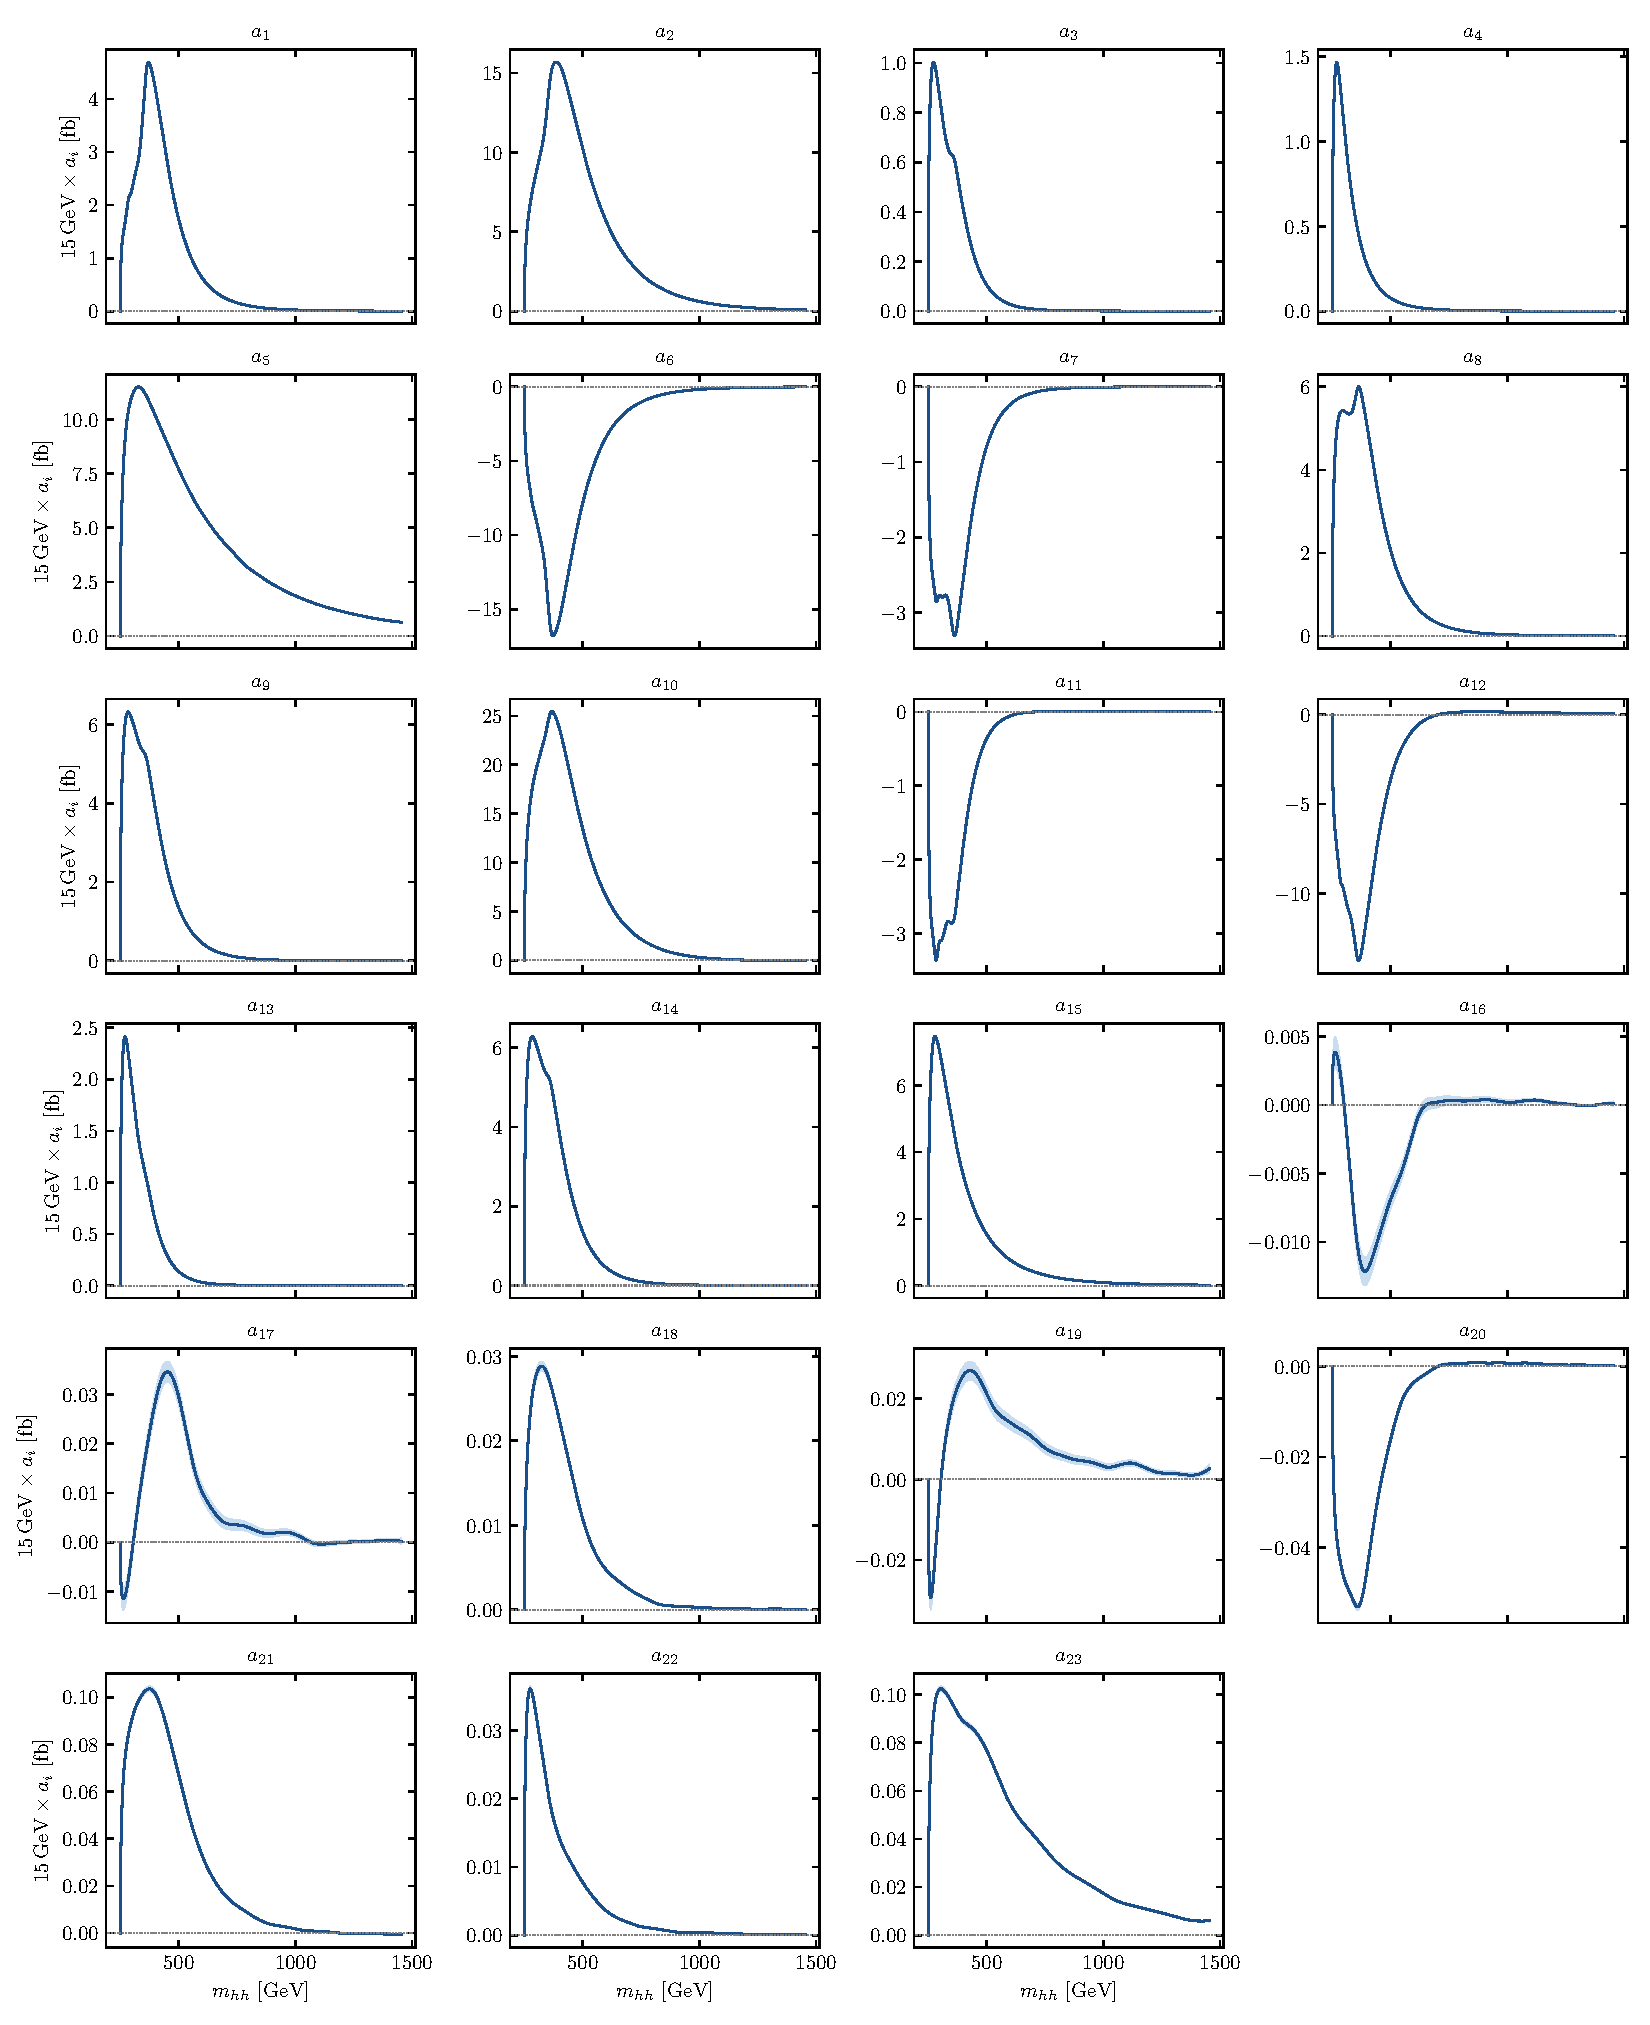
\includegraphics[width=\textwidth]{fig_A_coefficients.pdf}
\caption{The 23 coefficient functions $a_i(m_{hh})$, shown as $15\,\text{GeV}\times a_i$ (the cross section per
15~GeV multiplying the monomial $C_i(\theta)$ in each panel), with their exact $\pm1\sigma$ bands. Units are fb.}
\label{fig:A:coefficients}
\end{figure}

\subsection{Using the model}
\label{app:A:use}

The model consists of the breakpoints, the posterior mean $\hat{\boldsymbol\beta}$ and covariance $H^{-1}$, the 23
smoothness strengths and the three parameters of $\varepsilon(m)$, in one file, with a short Python module that
evaluates it; it requires only NumPy and SciPy~\cite{dihiggs:github}. For a HEFT point $\theta$ and any binning within
250--1455~GeV it returns the cross section in each bin with its fit uncertainty and model-error term. For a single
15~GeV bin the two are added in quadrature. For a sum over many bins the fit uncertainty is obtained exactly from
$H^{-1}$, while the model-error term lies between the limits of independent bins, $(\sum_k s^2_{\text{model},k})^{1/2}$,
and fully correlated bins, $\sum_k s_{\text{model},k}$. For the SM in 255--1455~GeV, for example,
$\sigma = 28.11$~fb, with a fit uncertainty of 0.006~fb and a model-error term between 0.03 and 0.17~fb. The
density itself, on scales finer than a 15~GeV bin just above threshold, is less certain than its band suggests
(appendix~\ref{app:B:results}).
